\documentclass[a4paper,11pt]{jsarticle}
\usepackage{graphicx}
\usepackage{wrapfig}
\usepackage{amsmath,amssymb,amsthm}
\usepackage{amssymb}
\usepackage{ascmac}
\usepackage{subfigure}
\usepackage{bm}
\usepackage{setspace}
\usepackage{cases}%左かっこつけるときに必要だった
\usepackage{leftidx}%行列表示用?
\usepackage{fancyhdr}
\usepackage{graphicx}
\usepackage{float}
\usepackage{booktabs}

\setlength{\headsep}{5mm}
\setlength{\oddsidemargin}{-0.5zw} %→にズラす
\setlength{\textheight}{37\baselineskip}
\addtolength{\textheight}{\topskip}
\setlength{\topmargin}{-10mm}
\setlength{\textwidth}{45zw} %文章の幅
\setlength{\textheight}{215mm}
\setlength{\parindent}{1zw}%箇条書きの一文字下げ
\pagestyle{fancy}

\theoremstyle{definition} \newtheorem{law}{定理}
\renewcommand{\proofname}{証明} 
\newcommand{\argmax}{\mathop{\rm arg~max}\limits}
\newcommand{\argmin}{\mathop{\rm arg~min}\limits}

\lhead{CVaR を用いるポートフォリオ最適化問題}
\chead{}
\rhead{総合ゼミ}
\lfoot{チョウ シホウ}
\cfoot{\thepage}
\rfoot{5月22日}
\renewcommand{\footrulewidth}{0.4pt}
\title{CVaR を用いるポートフォリオ最適化問題}
\author{12M42340 チョウ シホウ}
\date{5月22日}

\begin{document}
%\pagenumbering{roman}
%\tableofcontents
%\cleardoublepage
\pagenumbering{arabic}
\renewcommand{\thepart}{\arabic{part}}
\maketitle
\thispagestyle{empty}
\begin{abstract}
卒論ではCVaRリスク測度を紹介し,CVaRを用いるポートフォリオ最適化を利用して中国の株式市場で検証を行った上,リスクマネジメントの改善策を論じていた.今回は卒論の内容をアレンジして最適化の観点からCVaRを用いるポートフォリオ最適化の説明を行う.
\end{abstract}
\section{導入:ポートフォリオ最適化問題}
投資を行う際,投資家はリターンを追い求めるだけでなく,それに伴うリスクを定量的に管理する必要がある.一般的に複数の銘柄に投資を行うことによってリスクを軽減することができるため,投資家は分散投資を行う,投資家にとって最適な資産分配(ポートフォリオ)を決定する問題をポートフォリオ最適化問題といい,それを解くために様々な数理モデルが提案されている.その中に最も有名なのはMarkowitzの平均・分散モデルである.
\begin{equation}
\begin{split}
\text{min\,\,\,\,\,\,\,} & x^TAx \\
\text{s.t.\,\,\,\,\,\,\,} & y^Tx = \rho \\
& x^Te = 1 \\
& x \ge 0, x \in \mathbb{R}^n
\end{split}
\end{equation}
だだし,収益率ベクトル$y \in \mathbb{R}^n$,投資比率ベクトル$x \in \mathbb{R}^n$,分散共分散行列$A \in  \mathbb{R}^n\times\mathbb{R}^n$,$e=(1,1,\dots,1)^T,e \in \mathbb{R}^n$,無リスク資産なし,空売り不可.投資者はリスク回避的な立場を取る(期待収益率は大きいほど望ましい,収益のリスクは小さいほど望ましい).

\section{Value-at-Risk}
\subsection{定義}
投資対象の銘柄を$i=1,\dots,n$とし,銘柄$i$に対する投資比率を$x_i$,銘柄$i$の収益率を$y_i$とする,ここで,$y_i$は確率変数であり,以下では$x=(x_1,\dots,x_n)^T,y=(y_1,\dots,y_n)^T$と表す,損失関数を$f(x,y)$とし,確率変数$y$は連続的な確率密度関数$p(y)$に従うと仮定する.損失が$\zeta$以下となる確率を
\begin{equation}
\Psi(x,\zeta) = \int_{f(x,y)\le\zeta} p(y)dy
\end{equation}
で与える.VaRとはあるポートフォリオの損失が$\zeta$以下である確率が$\alpha$以上となるときの最小の$\zeta$,すなわち
\begin{equation}
\text{VaR}_{\alpha}(x) = \zeta_{\alpha}(x) = \min\{  \zeta | \Psi(x,\zeta) \ge \alpha \}
\end{equation}
と定義される.
\subsection{VaRの問題点}
$X$を確率変数とし,あるリスク尺度を$\rho(X)$とする.次の四つの性質を満たすリスク尺度はCoherent measures of riskと呼ばれる.
\begin{enumerate}
\item 単調性(monotonicity):$X_1 \le X_2$ならば$\rho(X_1) \le \rho(X_2)$
\item 劣加法性(subadditivity):$\rho(X_1 + X_2) \le \rho(X_1) + \rho(X_2)$
\item 正斉次性(positive homogeneity):$\forall \lambda > 0, \rho(\lambda X) = \lambda\rho(X)$
\item 平行移動不変性(translation invariance):$\forall c \in \mathbb{R},\rho(X+c)=\rho(X)+c$
\end{enumerate}
VaRはリスク尺度として単調性,正斉次性,平行移動不変性は満たすが劣加法性は満たさない.

\section{Conditional Value-at-Risk}
\subsection{CVaRの定義}
条件付きVaR(Conditional Value-at-Risk)とはあるポートフォリオの損失が$\zeta_{\alpha}(x)$を上回る場合の損失の期待値であり,
\begin{equation}
\text{CVaR}_{\alpha}(x) = \phi_{\alpha}(x)= \frac{\int_{f(x,y) \ge \zeta_{\alpha}(x)} f(x,y)p(y)dy}{\int_{f(x,y) \ge \zeta_{\alpha}(x)} p(y)dy}
\end{equation}
で定義される,$\int_{f(x,y) \ge \zeta_{\alpha}(x)} p(y)dy = 1- \alpha$となるため,CVaRは
\begin{equation}
\phi_{\alpha}(x) = \frac{1}{1-\alpha} \int_{f(x,y) \ge \zeta_{\alpha}(x)} f(x,y)p(y)dy \label{CVAREQU}
\end{equation}
と書き換える.CVaRはVaRを上回る場合の損失の期待値であるから明らかに次の不等式が成り立つ.
\begin{equation}
\zeta_{\alpha}(x) \le \phi_{\alpha}(x)
\end{equation}
一方,確率変数$y$が正規分布に従うという仮定がないならば,$\zeta_{\alpha}(x)$を最小にする$x$と$\phi_{\alpha}(x)$は同じであるとは限らない.
\subsection{CVaRの凸性}

\begin{law}
$X$と$Y$を連続な分布関数を持つ確率変数とするとき,任意の$\alpha \in (0,1)$に対して確率水準$\alpha$でのCVaRは以下の劣加法性を満たす.
\begin{equation}
\phi_{\alpha}(X+Y) \le \phi_{\alpha}(X) + \phi_{\alpha}(Y)
\end{equation}
\end{law}

\begin{proof}
$Z =  X + Y$とする.損失額$X$の$\alpha$分位点を$x_{\alpha}$,$Y$の$\alpha$分位点を$y_{\alpha}$,$Z$の$\alpha$分位点を$z_{\alpha}$とすると,
\begin{equation}
\begin{split}
\phi_{\alpha}(X) = & \frac{1}{1-\alpha} E[X1_{X \ge x_{\alpha}}] \\
\phi_{\alpha}(Y) = & \frac{1}{1-\alpha} E[Y1_{Y \ge y_{\alpha}}] \\
\phi_{\alpha}(Z) = & \frac{1}{1-\alpha} E[Z1_{Z \ge z_{\alpha}}]
\end{split}
\end{equation}
ただし,$1_A$は$A$の指示関数である.また,
\begin{equation}
\begin{cases}
1_{X \ge x_{\alpha}} - 1_{Z \ge z_{\alpha}} \ge 0 & \text{\,\,\,if\,\,\,} X \ge x_{\alpha} \\
1_{X \ge x_{\alpha}} - 1_{Z \ge z_{\alpha}} \le 0 & \text{\,\,\,if\,\,\,} X \le x_{\alpha} \\
\end{cases}
\end{equation}
という関係が成立するので$ (1_{X \ge x_{\alpha}} - 1_{Z \ge z_{\alpha}})(X - x_{\alpha})  \ge 0$となる,同様に$ (1_{Y \ge y_{\alpha}} - 1_{Z \ge z_{\alpha}})(Y - y_{\alpha})  \ge 0$,すると,
\begin{equation*}
\begin{split}
&(1-\alpha)(\phi_{\alpha}(X) + \phi_{\alpha}(Y) - \phi_{\alpha}(Z))\\
= & \,\, E[X1_{X \ge x_{\alpha}} + Y1_{Y \ge y_{\alpha}} - Z1_{Z \ge z_{\alpha}}] \\
= & \,\, E[X(1_{X \ge x_{\alpha}} - 1_{Z \ge z_{\alpha}}) + Y(1_{Y \ge y_{\alpha}} - 1_{Z \ge z_{\alpha}})] \\
\ge  & \,\,  x_{\alpha}E[1_{X \ge x_{\alpha}} - 1_{Z \ge z_{\alpha}}] + y_{\alpha}E[1_{Y \ge y_{\alpha}} - 1_{Z \ge z_{\alpha}}] \\
= & \,\, 0
\end{split}
\end{equation*}
したがって,$\phi_{\alpha}(X+Y) \le \phi_{\alpha}(X) + \phi_{\alpha}(Y)$が成り立つ.
\end{proof}

\begin{law}
あるリスク尺度が正斉次性を満たす場合,そのリスク尺度が劣加法性を満たすことと凸性を満たすことは同値である.
\end{law}
\begin{proof}
略
\end{proof}

\section{CVaRを用いるポートフォリオ最適化問題}
\subsection{準備}
$f(x,y) \ge \zeta_{\alpha}(x)$が成立するので,式\ref{CVAREQU}で定義した$\phi_{\alpha}(x)$を求めるためにパラメーター$\zeta \in \mathbb{R}$を用いて補助関数
\begin{equation}
F_{\alpha}(x,\zeta) = \zeta + \frac{1}{1-\alpha}\int_{y \in \mathbb{R}^n } [f(x,y)-\zeta]^+p(y)dy
\end{equation}
に定める.この時,$[t]^+ = \max\{0,t\}$である.$\phi_{\alpha}(x)$と補助関数$F_{\alpha}(x,\zeta)の間に以下の関係が成り立つ$.
\begin{law}
任意に固定した$x$に対して$F_{\alpha}(x,\zeta)$は$\zeta$の関数として凸かつ連続的微分可能であり,$\phi_{\alpha}(x)$は$F_{\alpha}(x,\zeta)$を$\alpha$に関して最小化することにより与えられる.つまり,
\begin{equation}
\phi_{\alpha}(x) = \min_{\zeta \in \mathbb{R}} F_{\alpha}(x,\zeta)
\end{equation}
である.また,上記の式の右辺の最小値を与える$\alpha$の集合を
\begin{equation}
A_{\alpha}(x) = \argmin_{\zeta \in \mathbb{R}} F_{\alpha}(x,\zeta)
\end{equation}
とすると$A_{\zeta}(x)$は空ではない閉空間となるので,その左辺の点$\zeta_{\alpha}(x)$は
\begin{equation}
\zeta_{\alpha}(x) \in \argmin_{\zeta \in \mathbb{R}} F_{\alpha}(x,\zeta), \,\,\,\,\, \phi_{\alpha}(x) = F_{\alpha}(x,\zeta_{\alpha}(x))
\end{equation}
である.
\end{law}
\begin{proof}
\cite{wardi}により,固定した$x$に対して$G(\zeta)=\int_{y \in \mathbb{R}^m [f(x,y)-\zeta]^+ p(y)dy}$と定めると$G$は凸で微分可能であり$G'(\zeta)=\Psi(x,\zeta) -1$が成り立つ.$F_{\alpha}(x,\zeta)$は$\zeta$に関して凸かつ微分可能であり,
\begin{equation}
\frac{d}{d\zeta} F_{\alpha}(x,\zeta) = \frac{1}{1- \alpha}(\Psi(x,\zeta)-\alpha)
\end{equation}
が成立.これにより,$F_{\alpha}(x,\zeta)$の最小値を与える$\zeta$は$\Psi(x,\zeta)=\alpha$を満たす$\zeta$となる.$\Psi(x,\zeta)$は連続で$\zeta \to \infty$で$1$となり,$\zeta \to -\infty$で$0$となる$\zeta$に関して非減少な関数であるから$A_{\alpha}(x)$は空集合でない閉集合となる.また,
\begin{equation}
\min_{\zeta \in \mathbb{R}}F_{\alpha}(x,\zeta) = F_{\alpha}(x,\zeta_{\alpha}(x)) = \zeta + \frac{1}{1-\alpha}\int_{y \in \mathbb{R}^n } [f(x,y)-\zeta]^+p(y)dy
\end{equation}
となり,右辺の積分は
\begin{equation}
\int_{f(x,y) \ge \zeta_{\alpha}(x)}[f(x,y) - \zeta_{\alpha}(x)]p(y)dy = \int_{f(x,y) \ge \zeta_{\alpha}(x)} f(x,y)p(y)dy - \zeta_{\alpha}(x) \int_{f(x,y) \ge \zeta_{\alpha}(x)} p(y)dy
\end{equation}
と変形できる.さらに,右辺の第1項は定義より$(1-\alpha)\phi_{\alpha}(x)$,第二項は$(1-\alpha)\zeta_{\alpha}(x)$となるため,
\begin{equation}
\min_{\zeta \in \mathbb{R}} F_{\alpha}(x,\zeta) = \zeta_{\alpha}(x) + \frac{1}{1-\alpha}[(1-\alpha)\phi_{\alpha}(x)-(1-\alpha)\zeta_{\alpha}(x)] = \phi_{\alpha}(x)
\end{equation}
である.
\end{proof}

\begin{law}
$\phi_{\alpha}(x)$を$x \in X$について最小化することと,$F_{\alpha}(x,\zeta)$を$(x,\zeta) \in X \times \mathbb{R}$に関して最小化することは等価である.つまり,
\begin{equation}
\min_{x \in X} \phi_{\alpha}(x) = \min_{(x,\zeta) \in X \times \mathbb{R}} F_{\alpha}(x,\zeta)
\end{equation}
さらに,$f(x,y)$が$x$に関して凸ならば$F_{\alpha}(x,\zeta)$は$(x,\zeta)$に関して凸であり,$\phi_{\alpha}$は$x$に関して凸である.
\end{law}
\begin{proof}
略
\end{proof}
次は,CVaRを用いるポートフォリオ最適化問題を線形計画問題として定式化する.
\subsection{線形計画問題}
密度関数$p(y)$に従う確率変数$y$をサンプルすることにより,補助関数$F_{\alpha}(x,\zeta)$の近似を行う.サンプリングによって$\{y_1,y_2,\dots,y_J\}$が得られた時,補助関数$F_{\alpha}(x,\zeta)$は以下のように近似される.
\begin{equation}
\bar{F}_{\alpha}(x,\zeta) =  \zeta + \frac{1}{1-\alpha} \sum_{j=1}^J \pi_j [f(x,y_j) - \zeta]^+
\end{equation}
ここで,$\pi_j$は$y_j$が得られる確率である.また,$f(x,y)$が連続であれば,$\bar{F}_{\alpha}(x,\zeta)$は凸かつ線形区分関数である.\\
さらに,$z_j,j=1,2,\dots,J$を定義する,$\bar{F}_{\alpha}(x,\zeta) $は
\begin{equation}
\bar{F}_{\alpha}(x,\zeta) =  \zeta + \frac{1}{1-\alpha} \sum_{j=1}^J \pi_j z_j
\end{equation}
に変形し,次の線形制約ができる.
\begin{equation}
z_j \ge  f(x,y_j) - \zeta, \,\,\, z_j \ge 0,\,\,\, j= 1,2,\dots,J, \,\,\, \zeta \in \mathbb{R}
\end{equation}
以上より,リスク尺度にCVaRを用いるポートフォリオ最適化問題は$\bar{F}_{\alpha}(x,\zeta)$の$(x,\zeta)  \in X \times \mathbb{R}$上での最小化問題として定式化できる.
\begin{eqnarray}
\text{min\,\,\,\,} && \bar{F}_{\alpha}(x,\zeta) =  \zeta + \frac{1}{1-\alpha} \sum_{j=1}^J \pi_j z_j \\
\text{s.t. \,\,\,\,} &&  z_j \ge  f(x,y_j) - \zeta, \,\,\, z_j \ge 0,\,\,\, j= 1,2,\dots,J, \,\,\, \zeta \in \mathbb{R}
\end{eqnarray}
一方,ポートフォリオの収益は各銘柄への投資比率とその銘柄の収益の積の総和として表されるので,損失関数は
\begin{equation}
f(x,y) = -x^Ty
\end{equation}
と定義される.また,投資家が最低限要求するリターンの期待値を$\rho$とすると次の条件が成立しなければならない.
\begin{equation}
x^T\bar{y} \ge \rho
\end{equation}
ただし,$\bar{y}$は収益率$y$の平均を表すベクトル.次にポートフォリオが満たすべき制約条件$x \in X$について考える,$x$ほ投資比率であり,空売り不可を仮定すると,
\begin{equation}
e^Tx = 1
\end{equation}
\begin{equation}
x \ge 0
\end{equation}
従って,CVaRを用いるポートフォリオ最適化問題は以下のように書ける.
\begin{eqnarray}
\text{min\,\,\,\,} && \bar{F}_{\alpha}(x,\zeta) =  \zeta + \frac{1}{1-\alpha} \sum_{j=1}^J \pi_j z_j \\
\text{s.t. \,\,\,\,} &&  z_j \ge  f(x,y_j) - \zeta, \,\,\, z_j \ge 0,\,\,\, j= 1,2,\dots,J, \,\,\, \zeta \in \mathbb{R} \\
&& x^T\bar{y} \ge \rho \\
&& e^Tx = 1 \\
&& x \ge 0
\end{eqnarray}

\section{Case study}
\subsection{中国株式市場の収益率分布}
上証50指数と深セン総合指数はそれぞれ上海証券取引所と深セン証券取引所のパフォーマンスを表す指数(インデックス)である.収益率$r_t = \log p_{t+1} - \log p_t$に定義する.
\begin{figure}[H]
\begin{minipage}[t]{0.45\linewidth}

 \begin{center}
  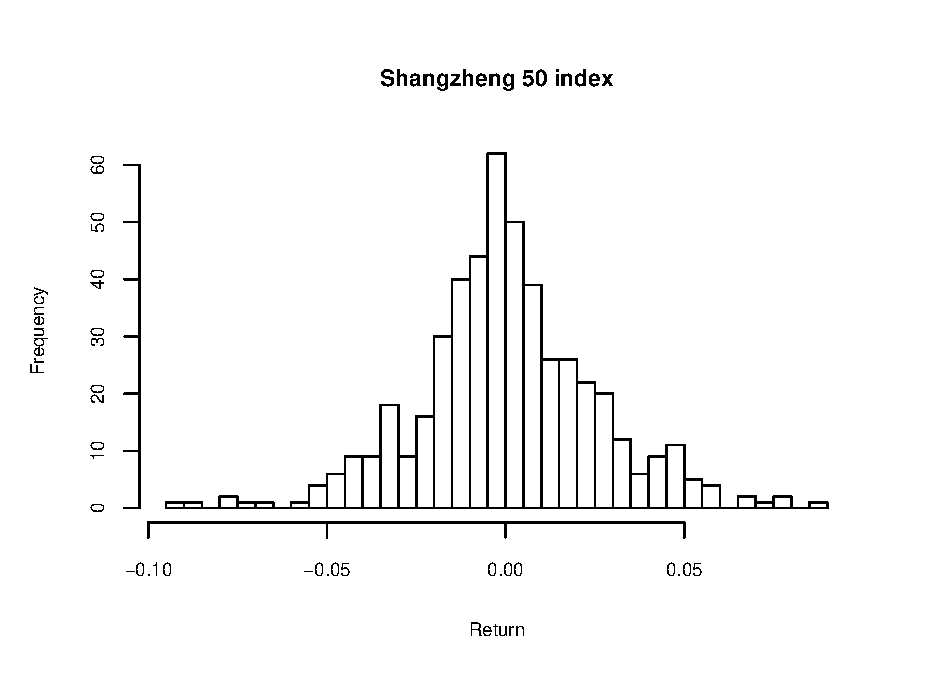
\includegraphics[width=70mm]{hist_sh50.eps}
 \end{center}
 \caption{上証50指数}
 \label{fig:one}
\end{minipage}
\begin{minipage}[t]{0.45\linewidth}
 \begin{center}
  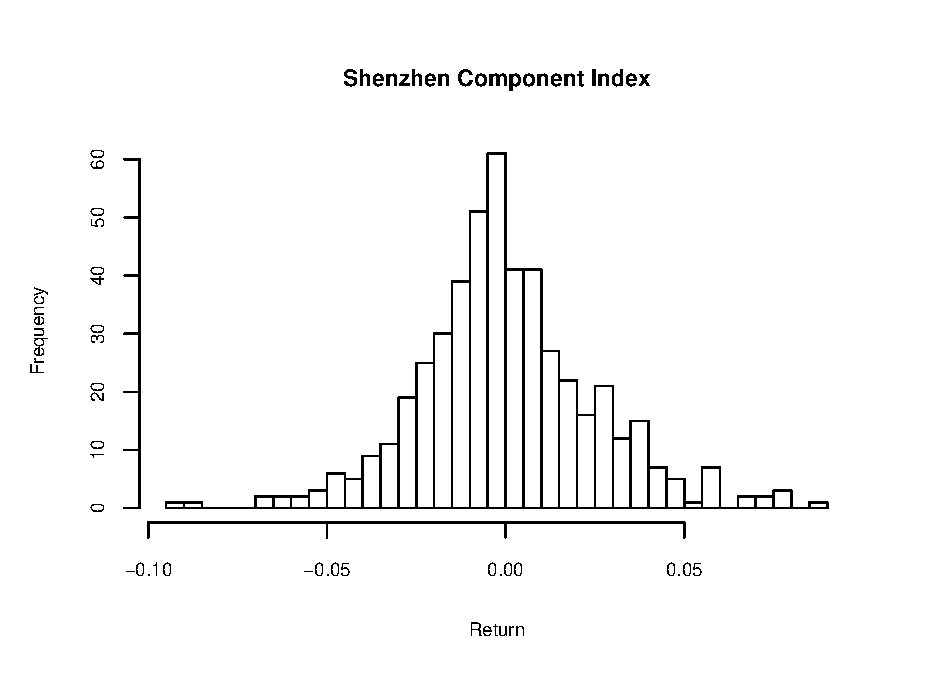
\includegraphics[width=70mm]{hist_szcf.eps}
 \end{center}
 \caption{深セン総合指数}
 \label{fig:one}
\end{minipage}
\end{figure}
次は,それらの対数収益率分布が正規分布に近似しているのかを検証する.対数収益率が正規分布に従ったら,歪度が$0$,尖度が$3$である.また,有意水準$0.01$の$\chi_2^2 = 9.21$ので,上証50指数と深セン総合指数の対数収益率は正規分布ではない.
\begin{table}[H]
\caption{収益率分布の分析}
\begin{tabular}{lcccccc}
\toprule
& 平均 & 分散 & 歪度 & 尖度 & Jarque-Bera Test \\
\midrule
上証50指数 & $0.0004879121$ & $0.000631557$ & $0.006364154$ & $1.136507$ & $27.1663$ \\
深セン総合指数 & $0.0001639911$ & $0.000627939$ & $0.213003300$ & $1.139042$ & $	31.0110$ \\
\bottomrule
\end{tabular}
\end{table}
\subsection{中国株式市場におけるポートフォリオ最適化}
\begin{figure}[H]
\begin{minipage}[t]{0.45\linewidth}
 \begin{center}
  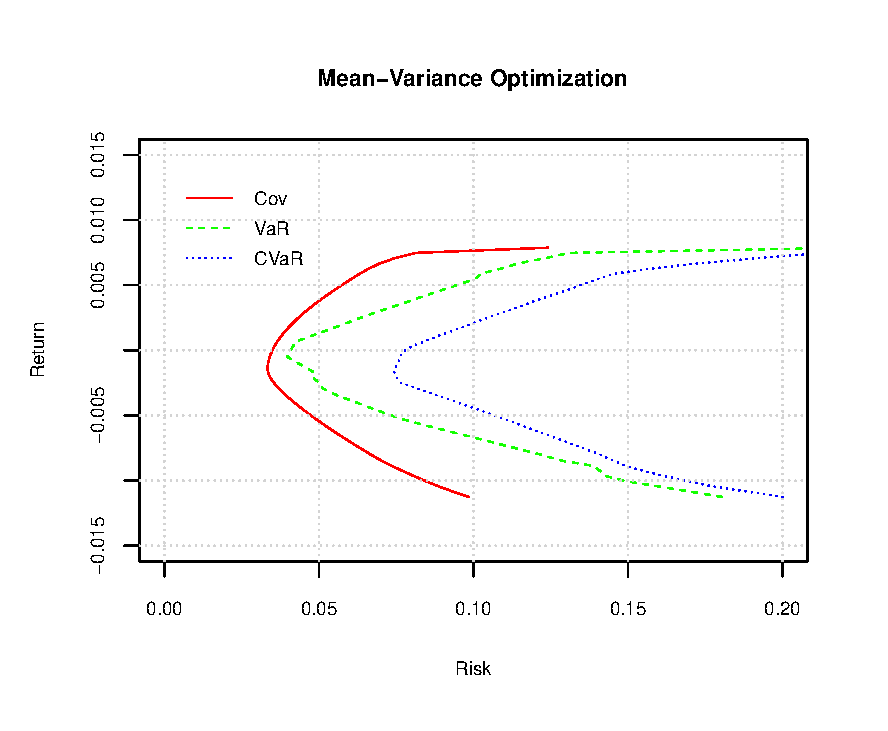
\includegraphics[width=70mm]{sh50_mvo.eps}
 \end{center}
 \caption{上証50指数・MVO}
 \label{fig:one}
\end{minipage}
\begin{minipage}[t]{0.45\linewidth}
 \begin{center}
  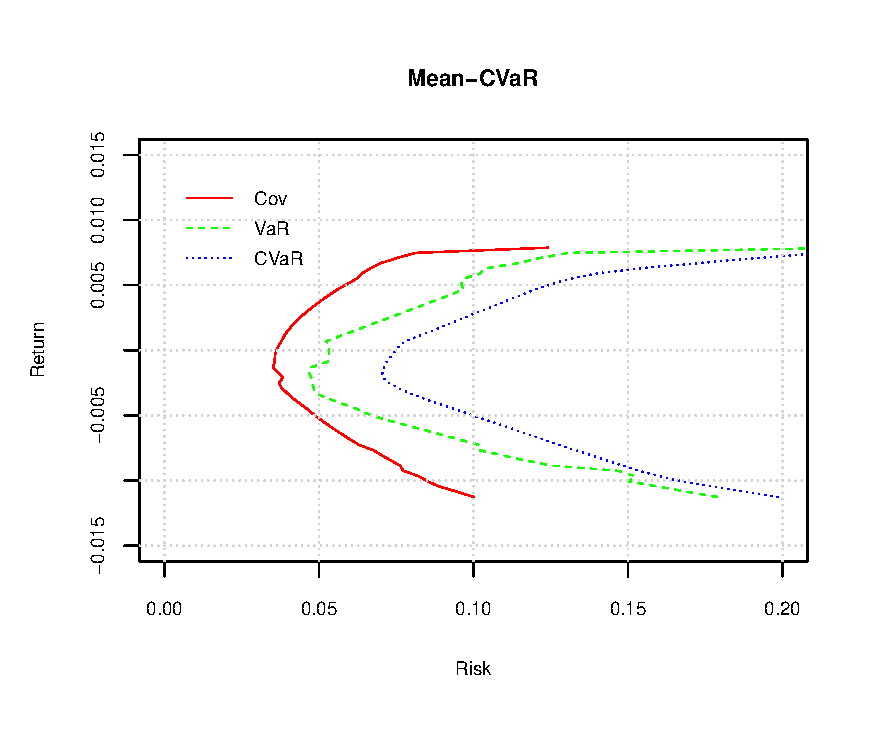
\includegraphics[width=70mm]{sh50_cvar.eps}
 \end{center}
  \caption{上証50指数・Mean-CVaR}
 \label{fig:one}
\end{minipage}
\end{figure}
\begin{figure}[H]
\begin{minipage}[t]{0.45\linewidth}

 \begin{center}
  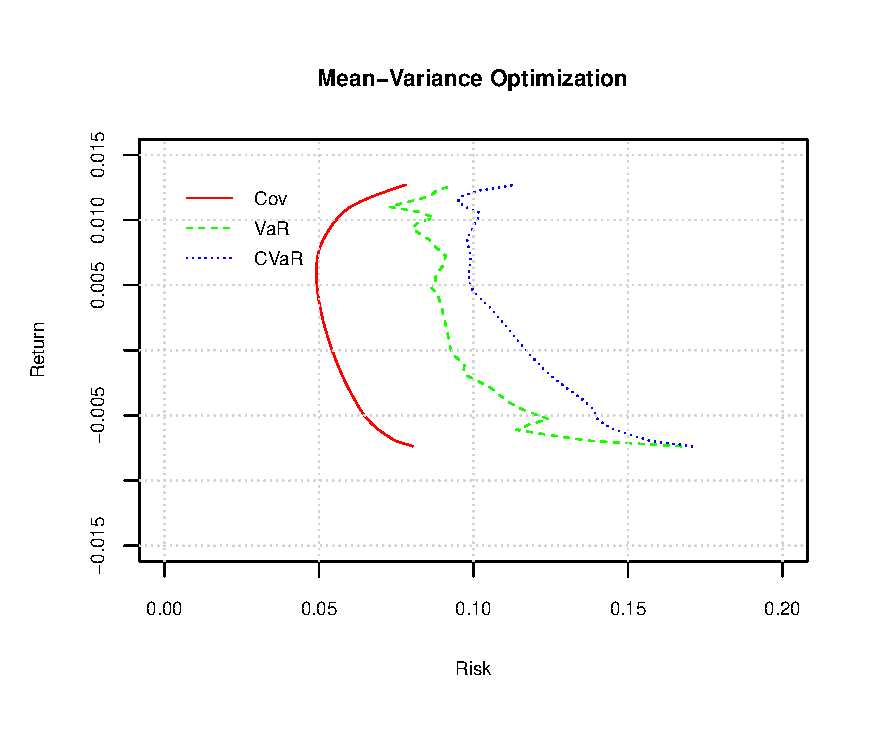
\includegraphics[width=70mm]{szcf_mvo.eps}
 \end{center}
 \caption{深セン総合指数・MVO}
 \label{fig:one}
\end{minipage}
\begin{minipage}[t]{0.45\linewidth}
 \begin{center}
  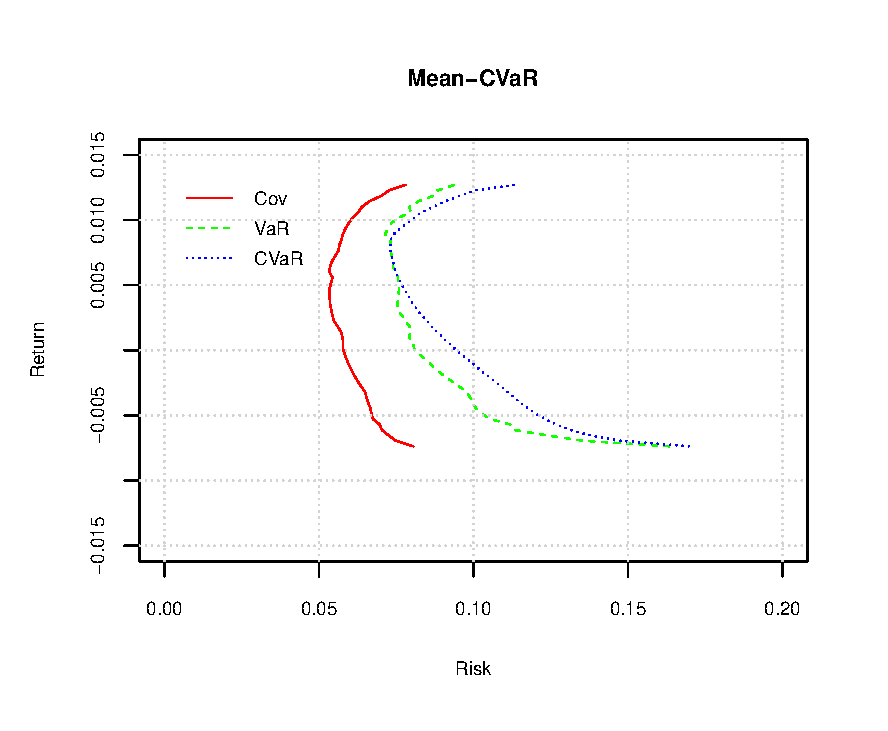
\includegraphics[width=70mm]{szcf_cvar.eps}
 \end{center}
 \caption{深セン総合指数・Mean-CVaR}
 \label{fig:one}
\end{minipage}
\end{figure}
\begin{itemize}
\item 期間:03/24/2008-03/25/2010
\item 銘柄:上証50指数の構成銘柄35銘柄(A株)と深セン総合指数の構成銘柄35銘柄(A株)
\item 収益率:対数収益率
\end{itemize}
\begin{table}[H]
\caption{上証50指数構成銘柄の効率的フロンティア}
\begin{center}
\begin{tabular}{lllllll}
\toprule
&\multicolumn{3}{c}{MVO} & \multicolumn{3}{c}{Mean-CVaR} \\
\cmidrule(r){2-4} \cmidrule(r){5-7}
收益率 & Cov &VaR	&CVaR &Cov &VaR &CVaR \\
\midrule
$0.1\%$	& $	0.0375$	& $	0.0464$	& $	0.0875$	& $	0.0385$	& $	0.0557$	& $	0.0813$\\
$0.2\%$	& $	0.0412$	& $	0.0579$	& $	0.0989$	& $	0.0417$	& $	0.0670$	& $	0.0918$\\
$0.3\%$	& $	0.0457$	& $	0.0695$	& $	0.1105$	& $	0.0463$	& $	0.0784$	& $	0.1023$\\
$0.4\%$	& $	0.0512$	& $	0.0820$	& $	0.1226$	& $	0.0518$	& $	0.0897$	& $	0.1128$\\
$0.5\%$	& $	0.0574$	& $	0.0945$	& $	0.1347$	& $	0.0584$	& $	0.0962$	& $	0.1242$\\
\bottomrule
\end{tabular}
\end{center}
\end{table}
\begin{table}[H]
\caption{深セン総合指数構成銘柄の効率的フロンティア}
\begin{center}
\begin{tabular}{lllllll}
\toprule
&\multicolumn{3}{c}{MVO} & \multicolumn{3}{c}{Mean-CVaR} \\
\cmidrule(r){2-4} \cmidrule(r){5-7}
收益率 & Cov &VaR	&CVaR &Cov &VaR &CVaR \\
\midrule
$0.6\%$	& $0.0491$ & 	$0.0883$ &	$0.0985$ &	$0.0534$ & 	$0.0749$ &	$0.0749$\\ 
$0.7\%$	& $0.0494	$ & 	$0.0907$ & 	$0.0991$ & 	$0.0546$ & 	$0.0738$ & 	$0.0738$\\
$0.8\%$	& $0.0505	$ & 	$0.0874$ & 	$0.0984$ & 	$0.0565$ & 	$0.0731$ & 	$0.0731$\\
$0.9\%$	& $0.0526	$ & 	$0.0823$ & 	$0.0989$ & 	$0.0579$ & 	$0.0715$ & 	$0.0746$\\
$1.0\%$	& $0.0555	$ & 	$0.0848$ & 	$0.1012$ & 	$0.0603$ & 	$0.0741$ & 	$0.0797$\\
\bottomrule
\end{tabular}
\end{center}
\end{table}
\section{今後}
とりあえず機械学習を学び,金融以外の分野で取り込んでみたい.
\begin{thebibliography}{99}
\bibitem{Risk} Philippe Artzner, Freddy Delbaen, Jean-Marc Eber and David Heath: Coherent Measures of Risk, Math. Finance 9 (1999), no. 3, 203-228
\bibitem{Opt} Krokhmal, Pavlo, Jonas Palmquist, and Stanislav Uryasev. Portfolio optimization with conditional value-at-risk objective and constraints. Portfolio The Magazine Of The Fine Arts 4.352 (2001) : 1-30.
\bibitem{OCVaR} Rockafellar, R. T. and S. Uryasev. Optimization of conditional value-at-risk. Journal of Risk 2 (2000): 21-41. 
\bibitem{wardi} Wardi, Y. \& Shapiro, A., 1994. Nondifferentiability of the Steady-State Function in Discrete Event Dynamic Systems. IEEE Transactions on Automatic Control, 39(8), p.1707-1711.
\end{thebibliography}
\end{document}